\documentclass[twocolumn]{article}
\usepackage{amsmath, amssymb, amsthm, bm}
\usepackage{graphicx, epsdice, xcolor, listings}
\usepackage[top=1.35in, bottom=1.35in, left=1.35in, right=1.35in]{geometry}

\newcommand{\EE}{\mathbb{E}}
\newcommand{\PP}{\mathbb{P}}
\newcommand{\RR}{\mathbb{R}}
%
\newcommand{\Dd}{\mathcal{D}}
\newcommand{\Ee}{\mathcal{E}}
\newcommand{\Gg}{\mathcal{G}}
\newcommand{\Hh}{\mathcal{H}}
\newcommand{\Ii}{\mathcal{I}}
\newcommand{\Kk}{\mathcal{K}}
\newcommand{\Ll}{\mathcal{L}}
\newcommand{\Ss}{\mathcal{S}}
\newcommand{\Tt}{\mathcal{T}}
\newcommand{\Uu}{\mathcal{U}}
\newcommand{\Vv}{\mathcal{V}}
\newcommand{\Xx}{\mathcal{X}}
\newcommand{\Yy}{\mathcal{Y}}

\newcommand{\Ein} {\text{trn}_{\Ss}} %{\Ee_{\text{in},\Uu}}
\newcommand{\Einb} {\text{trn}_{\check\Ss}} %{\Ee_{\text{in},\Uu}}
\newcommand{\Einc} {\text{trn}_{\Ss\sqcup \check\Ss}} %{\Ee_{\text{in},\Uu}}
\newcommand{\Egap}{\text{gap}_{\Ss}}
\newcommand{\Eout}{\text{tst}} %{\Ee_{\text{out}}}

\newtheorem{qst}{Question}
\newtheorem{thm}{Theorem}
\newtheorem{lem}{Lemma}
\theoremstyle{definition}
\newtheorem{dfn}{Definition}

\begin{document}

    \twocolumn[
        \begin{@twocolumnfalse}
            \begin{flushleft}  \Huge  \emph{What is...} \vspace{0.1cm}\\\hrule \end{flushleft}
            \begin{flushright} \Huge  Vapnik-Chervonenkis Dimension?     \end{flushright}
            \begin{flushright} \Large Samuel C.\ Tenka      \end{flushright}
        \end{@twocolumnfalse}
    ]

    \subsection*{The Cake Problem}

    Mathematicians and bakers alike know the sequence $1, 2, 4, 8, 16, \cdots$
    by heart.  It continues, of course, with $31$, for its $n$th element $p(n)$
    counts the pieces obtained from a disk-shaped cake by cutting along all
    ${n\choose 2}$ lines determined by $n$ points placed generically on the
    cake's perimeter.

    \begin{figure}[h!]
        \centering
        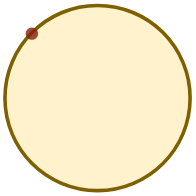
\includegraphics[height=2.3cm]{cake-1}
        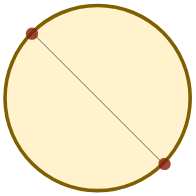
\includegraphics[height=2.3cm]{cake-2}
        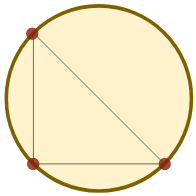
\includegraphics[height=2.3cm]{cake-3}
        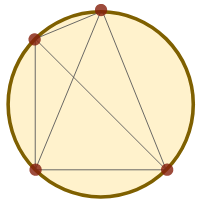
\includegraphics[height=2.3cm]{cake-4}
        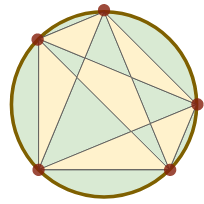
\includegraphics[height=2.3cm]{cake-5-col}
        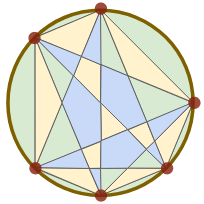
\includegraphics[height=2.3cm]{cake-6-col}
        \caption{\emph{
            Cakes for $n=1, \cdots, 6$.
            The $n=4$ cake (bottom left) has $p(4)=8$ pieces.  We
            color some pieces to make them easier to see and
            to count.  $p(6)$ is clearly odd: the
            pieces besides the central yellow triangle group into sets
            of six.
        }}
    \end{figure}

    Rather than growing exponentially, $p(n)$ is a polynomial.  
    We may compute $p(n)$ by regarding each sliced cake as a
    planar graph, observing that each interior point is determined by two
    cuts and hence by one of ${n\choose 4}$ many sets of $4$ perimeter
    points, and then applying Euler's polyhedron formula.  One finds that
    $p(n)$ is ${n-1 \choose 0}+\cdots+{n-1\choose 4}$, which explains
    why $p(n)$ initially coincides with $2^{n-1}$.

    This example, like many others in mathematics and in science, serves as a
    warning and a mystery: patterns do not always generalize.  But then ---
    \emph{how is generalizing from data possible at all}? 

    \subsection*{Learning and Generalization}

    In general, we wonder: \emph{if from a collection $\Hh$ of possible
    patterns we find some $f\in \Hh$ that matches $N$ observed data points,
    when should we expect that $f$ matches unseen data}?  This question
    motivates statistical learning theory and the foundations of machine
    learning.
    
    We may frame the problem in the setting of image classification,
    where $\Xx$ is a space of images, $\{\pm 1\} = \{\text{Cow}, \text{Dog}\}$ is
    a set of (for simplicity, two) labels, and we seek a classifier
    $f: \Xx\to\{\pm 1\}$ that accords with nature.
    More precisely, we posit a probability distribution $\Dd$ over the space
    $\Xx\times \{\pm 1\}$ of input-output pairs and we let $\Hh \subseteq \{\pm
    1\}^\Xx$ be a set of (measurable) functions.  If $\Ss \sim \Dd^N$ denotes a
    sequence of $N$ observations drawn independently from $\Dd$, the
    \textbf{in-sample error} of $f\in \Hh$ is 
    $$
        \Ein(f) = \PP_{(x,y)\sim \Ss}[f(x)\neq y] 
    $$
    and the \textbf{out-of-sample error} is 
    $$
        \Eout(f) = \PP_{(x,y)\sim \Dd}[f(x)\neq y] 
    $$
    A \textbf{learning rule} $\Ll: (\Xx\times\{\pm 1\})^N \to \Hh$ maps
    $\Ss$s to $f$s.  We wonder when a small in-sample error implies a
    small out-of-sample error, that is, when we may bound the
    \textbf{generalization gap} 
    $$
        \Egap(\Ll) = \Eout(\Ll(\Ss)) - \Ein(\Ll(\Ss)) 
    $$
    In degenerate cases where $\Ll(\Ss)$ and $\Ss$ are independent, $\Ein(\Ll(\Ss))$ is
    an unbiased estimator for $\Eout(\Ll(\Ss))$, and by laws of large numbers, $\Egap$ is
    small for large $N$.  We wonder: \emph{can we still control the gap when
    $\Ll(\Ss)$ depends on
    $\Ss$}?
    %
    \textbf{Vapnik-Chervonenkis theory} answers this question affirmatively for
    sufficiently nice $\Hh$.

    The two ingredients are \emph{concentration} and \emph{symmetrization}.

    \subsection*{Concentration of Measure}

    \begin{lem}[Chernoff]
        The fraction of heads among $N$ i.i.d.\ flips of a biased coin
        exceeds its mean $p$ by more than $g$ with probability at most 
        $\exp(-Ng^2)$, for all $p, g\in[0,1]$.
    \end{lem}

    \begin{proof}
            \begin{figure}[h!]
                \centering
                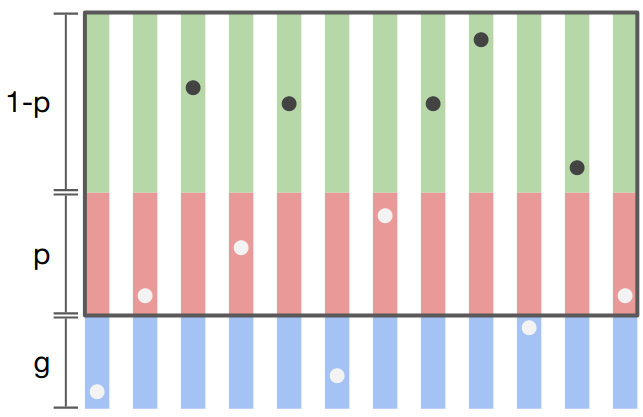
\includegraphics[height=4cm]{chernoff}
                \caption{\emph{
                    We randomly select points on $N$ vertical sticks.  Each
                    stick has three parts: \textbf{green} with length $1-p$,
                    \textbf{red} with length $p$, and \textbf{blue} with length
                    $g$.  We call non-blue points \textbf{boxed} and non-green
                    points \textbf{hollow}.
                }}
                \label{fig:chernoff}
            \end{figure}

            We'll switch viewpoints: flipping a coin is like choosing a boxed
            point on a stick where green means tails and red means heads (Figure \ref{fig:chernoff}).
            %
            We'll show that with high probability less than $M_0 = (p+g)N$
            flips heads.  That is --- given that all points are boxed --- less
            than $M_0$ points are red. 
            %
            For any $M\geq M_0$:
            \begin{align*}
                    & ~ \PP[\text{$M$ are red $\mid$ all are boxed}] \\
                  = & ~ \PP[\text{$M$ red and all are boxed}] ~/~ \PP[\text{all are boxed}]  \\
                  = & ~ \PP[\text{$M$ hollow}] \cdot
                        \frac{\PP[\text{all hollows are red $\mid$ $M$ hollow}]}{\PP[\text{all are boxed}]} \\
                  = & ~ \PP[\text{$M$ hollow}] \cdot (1+g/p)^{-M} ~/~ (1+g)^{-N} 
                %        \\
                %\leq& ~ \PP[\text{$M$ hollow}] \cdot
                %        (1+g/p)^{-M_0} ~/~ (1+g)^{-N} 
            \end{align*}
            Since the above holds for all $M\geq M_0$, the chance of too many
            heads is:
            \begin{align*}
                &~\PP[\text{at least $M_0$ are red $\mid$ all are boxed}] \\
                \leq
                &~(1+g/p)^{-M_0} / (1+g)^{-N}
            \end{align*}
            We finish by plugging in $M_0=(p+g)N$, bounding $1+x\leq \exp(x)$,
            and simplifying. 
    \end{proof}

    The Chernoff bound, proved above with suboptimal constants, is one of the  
    most basic \textbf{concentration inequalities}. 

    For any $f\in \Hh$, $\Ein(f)$ is the average of $N$ independent 
    Bernoullis of mean $\Eout(f)$.  So for $\Hh$ finite and $N$
    large, the gap is probably small:
    \begin{align*}
        &~\PP_{\Ss\sim \Dd^N}[\Egap(\Ll) \geq g] \\
        \leq 
        &~\sum_{f\in \Hh} \PP_{\Ss\sim \Dd^N}[\Ein(f) \geq \Eout(f) + g] \\
        \leq
        &~|\Hh| \cdot \exp(-Ng^2)
    \end{align*}

    For example, if $\Hh$ is parameterized by $P$ numbers, each represented on
    a computer by $32$ bits, then $|\Hh|\leq 2^P$ and, with probability
    $1-\delta$, the gap is no more than
    $$
        \sqrt{\log(2/\delta)\cdot 32 P/N}
    $$
    But shouldn't $32$ bits or $64$ bits or infinitely many bits yield similar
    behavior?  Intuitively, the $\Hh$s used in practice --- for instance,
    linear models or neural networks --- depend smoothly on their parameters;
    tiny changes in the parameters yield practically the same candidate, so
    $\Hh$'s cardinality is not an apt measure of its size.  As we will see, the
    V-C dimension measures $\Hh$ more subtly.

    \subsection*{Symmetrization}

    The key observation is that, even though $\Hh$ may be infinite,
    the restriction $\Hh_\Ss = \{f|_\Ss : f \in \Hh\}$ is finite for finite
    $\Ss$.  
    %
    So let us fix $f\in \Hh$ and estimate $\Eout(f)$ by $\Einb(f)$ for
    $(\Ss,\check\Ss) \sim\Dd^{2N}$ drawn independently. 
    By Chernoff, $\Eout$ and $\Einb$ are probably close:
    provided $g\geq 2/\sqrt{N}$,
    \begin{align*}
            ~& \PP[\Ein + g \leq \Eout]                              \\ 
        =   ~& \PP[\Ein + g \leq \Eout \mid \Eout \leq \Einb + g/2]  \\
        \leq~& \PP[\Ein + g/2 \leq \Einb \mid \Eout \leq \Einb + g/2]\\ 
        \leq~& \PP[\Ein + g/2 \leq \Einb] \cdot 2                     
    \end{align*}
    Imagining $\Ss$ as sampled \emph{without replacement} from
    $\Ss\sqcup\check\Ss$ and applying a variant of Chernoff, we find
    that $g \leq \Egap(\Ll)$ with chance at most
    \begin{align*}
        \max_{|\Ss|=|\check\Ss|=N}
        |\Hh_{\Ss\sqcup\check\Ss}| ~\cdot~ \exp(-Ng^2/16) \cdot 2
    \end{align*}

    Finally, to show that the gap is usually small, we need only bound
    $H(n) = \max_{|S|=n} |\Hh_S|$.

    Clearly, $H(n) \leq 2^n$.  In fact, this bound is never somewhat tight:
    depending on $\Hh$, it either is an equality or extremely loose!

    Indeed, consider $\Hh_S$ for $|S|=n$.  Ordering $S$,
    let us write each $f\in \Hh_S$ as a string of $+$s
    and $-$s.  To count these strings, we will first translate them from the
    alphabet $\{+,-\}$ to the alphabet $\{\blacksquare,\square\}$.
    %
    Intuitively, $\blacksquare$ represents ``surprisingly $+$''.
    More precisely, working from left to right, whenever two
    (partially translated) strings differ \textbf{only} in their
    leftmost untranslated coordinate we overwrite the $+$ version's
    $+$ by $\blacksquare$.  Otherwise, we overwrite by $\square$.

    \definecolor{moor}{rgb}{0.85,0.1 ,0.1 }
    \definecolor{moog}{rgb}{0.1 ,0.75,0.1 }
    \definecolor{moob}{rgb}{0.2 ,0.4 ,1.0 }
    \newcommand{\rR}[1]{{\color{moor}#1}}
    \newcommand{\gG}[1]{{\color{moog}#1}}
    \newcommand{\bB}[1]{{\color{moob}#1}}
    \newcommand{\E}{\texttt{$\square$}}
    \newcommand{\D}{\texttt{$\blacksquare$}}
    \newcommand{\A}{\texttt{$\bm{+}$}}
    \newcommand{\M}{\texttt{$\bm{-}$}}
    \begin{figure}[h]
        \centering
        \resizebox{\columnwidth}{!}{
            \begin{tabular}{ccccccccc}
                   \A \M \M \M  &       &  \E \gG\M \M \M  &       &  \E \E \rR\M \M  &       &  \E \E \E \rR\M  &       &  \E \E \E \E  \\
                   \M \A \M \M  &       &  \E \gG\A \M \M  &       &  \E \D    \M \M  &       &  \E \D \E \bB\M  &       &  \E \D \E \E  \\
                   \M \M \A \M  &       &  \E    \M \A \M  &       &  \E \E \rR\A \M  &       &  \E \E \D \gG\M  &       &  \E \E \D \E  \\
                   \M \M \M \A  & $\to$ &  \E    \M \M \A  & $\to$ &  \E \E \gG\M \A  & $\to$ &  \E \E \E \rR\A  & $\to$ &  \E \E \E \D  \\
                   \M \M \A \A  &       &  \E \bB\M \A \A  &       &  \E \E \gG\A \A  &       &  \E \E \D \gG\A  &       &  \E \E \D \D  \\
                \rR\M \A \A \A  &       &  \E \bB\A \A \A  &       &  \E \D    \A \A  &       &  \E \D \E \bB\A  &       &  \E \D \E \D  \\
                \rR\A \A \A \A  &       &  \D    \A \A \A  &       &  \D \E    \A \A  &       &  \D \E \E    \A  &       &  \D \E \E \E
            \end{tabular}
        }
        \caption{
            Translating elements of $H_S$ (left) to strings of choice points
            (right).  Each row corresponds to one of $7$ candidates and each
            column corresponds to one of of $4$ datapoints.
            %
            We color pairs of strings that differ at-and-only-at their leftmost
            untranslated coordinate.
        }
        \label{fig:sauer}
    \end{figure}

    Each step of translation keeps distinct strings distinct.
    %
    Moreover, whenever some $k$ indices $T\subseteq S$ of a translated string
    are $\blacksquare$s, $|\Hh_T| = 2^k$.  This is because $\blacksquare$s mark
    choice points where the candidates attain both $+$ and $-$.
    %
    Now, \textbf{either} $H(n)=2^n$ for all $n$, \textbf{or} $H(k+1) \neq 2^{k+1}$
    for some $k$.  In the latter case, no translated string may have $k$ or
    more $\blacksquare$s.  Thus $\Hh_S$ contains no more strings than
    there are subsets in $S$ of size $\leq k$.  Therefore,
    $$
        H(n)
        \leq 
        {n\choose 0} + {n\choose 1} + \cdots + {n\choose k}
        \leq 
        (n+2)^{k}
    $$
    As with Cake, what might grown as $2^n$ grows only
    polynomially.

    In short, if some $H(k+1) \neq 2^{k+1}$, then $\Egap(\Ll) \geq g$
    with chance at most
    $$
       (2N+2)^k \cdot \exp(-Ng^2/16) \cdot 2
    $$
    Because this tends to $0$ as $N$ grows, generalizing from data is possible.

    Since $k$ appears as an exponent, it is morally a measure of dimension:
    \begin{dfn}
        The \textbf{Vapnik-Chervonenkis dimension} of a set
        $\Hh \subseteq \{\pm 1\}^\Xx$ is the supremal $k$ for which
        $H(k) = \max_{|S|=k} |\Hh_S| = 2^k$.  
    \end{dfn}
    The following theorem, whose ``only if'' direction we have sketched above,
    highlights the V-C dimension's importance to learning theory:
    \begin{thm}[Vapnik and Chervonenkis, 1971]
        The V-C dimension of $\Hh$ is finite if and only if for all data
        distributions $\Dd$, learning rules $\Ll$, and gap bounds $g>0$, the
        chance that $\Egap(\Ll)$ exceeds $g$ tends to $0$ as $N=|\Ss|$ grows.  
    \end{thm}

    \subsection*{Statistical Learning Theory}

    \subsection*{References}
        The use of three-segment sticks and $\{\blacksquare,
        \square\}$-encoding to give short, elementary proofs of Chernoff's
        bound and the VC Theorem are, as far as the author knows, new.  That
        said, they correspond directly to classical proofs involving moment
        generating functions and induction on sums of binomial coefficients,
        respectively. 



%            We can solve for the gap in terms of our tolerance $\delta$.
%            If we call the (smallest) $k$ for which $H(k+1) \neq 2^{k+1}$
%            the \textbf{jaggedness}\footnote{
%                To recap, the jaggedness of $\Hh$ is the smallest $k$ such
%                that $\Hh$ fails to fit all $2^{k+1}$ many $\pm$ patterns
%                on each dataset $S$ of size $k+1$.
%                %
%                If no such $k$ exists, we say that $\Hh$ is infinitely jagged.
%                %
%                The jaggedness is also known as the \emph{Vapnik-Chervonenkis
%                dimension}.
%            } of $\Hh$, then what we get is:
%            $$
%                \Egap
%                \leq
%                \sqrt{\frac{16\log(2N+2) \cdot \text{jaggedness} + 16\log(2/\delta)}{N}}
%            $$
%
%            Here's an example.  Consider classifying rainfall levels as
%            ``desert'' or ``non-desert'' according to how they compare to
%            some positive real number $r$.  Each $r$ gives a different
%            candidate, so there are infinitely many candidates.  But for any
%            $k=2$ rainfall levels $a<b$, no candidate classifies $a$ but not
%            $b$ as ``desert''.  So $\Hh$ has jaggedness $2-1=1$.
%            %
%            In cases like these, where the jaggedness counts the parameters, we
%            have essentially replaced the $32$ (bits per parameter) by $\approx
%            \log(N)$.\footnote{
%                Due to the constants involved, this is in practice not a
%                substantial improvement.
%            } Intuitively, each parameter has $\approx \log(N)$ bits
%            relevant to distinguishing the datapoints; further bits are
%            irrelevant to overfitting.
%
%            Generalization thus stems from $\Hh$'s shape, not its literal size.
%            Unless $\Hh$ is infinitely jagged, the gap will shrink as $N$
%            grows.  In this case, learning from data is possible.
\end{document}


